\documentclass[aspectratio=169, 12pt]{beamer}
\usetheme{Madrid}
\usecolortheme{seahorse}

\usepackage[utf8]{inputenc}
\usepackage[T1]{fontenc}
\usepackage{lmodern}
\usepackage{listings}
\usepackage{graphicx}
\usepackage{tikz}
\usepackage{booktabs}
\usetikzlibrary{arrows.meta, positioning, fit, shapes.geometric, calc}

\lstset{
  basicstyle=\ttfamily\scriptsize,
  keywordstyle=\color{blue!70!black}\bfseries,
  stringstyle=\color{green!50!black},
  commentstyle=\color{gray},
  breaklines=true,
  frame=single,
  backgroundcolor=\color{gray!5},
  xleftmargin=4pt,
  xrightmargin=4pt,
  literate={<-}{$\leftarrow$}2,
}

\title{MAS Framework -- Walking Skeleton}
\subtitle{Cost-Efficient LLM-Based Multi-Agent Simulation}
\author{Janik H\"ausser}
\date{\today}

\begin{document}

% ============================================================
\begin{frame}
\titlepage
\end{frame}

% ============================================================
\begin{frame}{\"Uberblick: Was macht das System?}

\begin{center}
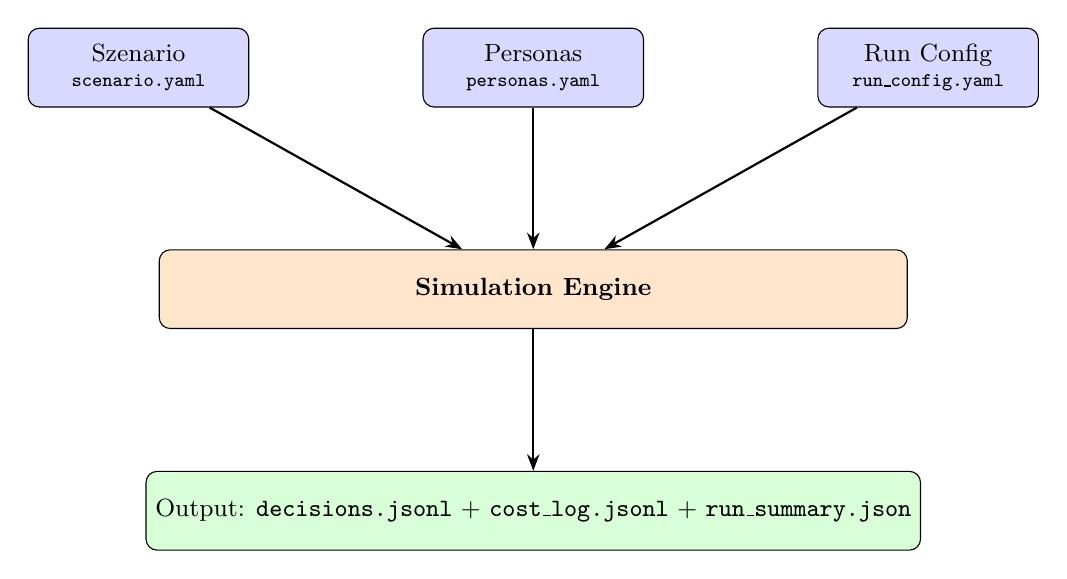
\begin{tikzpicture}[
    box/.style={draw, rounded corners, minimum width=2.8cm, minimum height=1cm, align=center, font=\small},
    arrow/.style={-{Stealth[length=6pt]}, thick},
    node distance=1.4cm and 2.2cm
]
    % Input layer
    \node[box, fill=blue!15] (scenario) {Szenario\\[-2pt]\scriptsize\texttt{scenario.yaml}};
    \node[box, fill=blue!15, right=of scenario] (personas) {Personas\\[-2pt]\scriptsize\texttt{personas.yaml}};
    \node[box, fill=blue!15, right=of personas] (runconfig) {Run Config\\[-2pt]\scriptsize\texttt{run\_config.yaml}};
    
    % Engine
    \node[box, fill=orange!20, below=1.8cm of personas, minimum width=9.5cm] (engine) {\textbf{Simulation Engine}};
    
    % Output
    \node[box, fill=green!15, below=1.8cm of engine, minimum width=9.5cm] (output) {Output: \texttt{decisions.jsonl} + \texttt{cost\_log.jsonl} + \texttt{run\_summary.json}};
    
    % Arrows
    \draw[arrow] (scenario) -- (engine);
    \draw[arrow] (personas) -- (engine);
    \draw[arrow] (runconfig) -- (engine);
    \draw[arrow] (engine) -- (output);
\end{tikzpicture}
\end{center}

\vspace{0.3cm}
\textbf{3 YAML-Dateien rein} $\rightarrow$ \textbf{strukturierte Ergebnisse raus}

\end{frame}

% ============================================================
\begin{frame}{Die drei Input-Dateien}

\begin{columns}[T]
\begin{column}{0.33\textwidth}
\textbf{scenario.yaml}\\[4pt]
\textit{Was} wird simuliert?
\begin{itemize}\small
    \item Rollen (Buyer, Seller)
    \item Runden (min/max)
    \item Interaktionstyp
    \item Sichtbarkeitsregeln 
    \item Incentive-Mechanismen
\end{itemize}
\end{column}

\begin{column}{0.33\textwidth}
\textbf{personas.yaml}\\[4pt]
\textit{Wer} simuliert?
\begin{itemize}\small
    \item Hintergrund/Bio
    \item Ziele (prim\"ar/sekund\"ar)
    \item Risikoprofil
    \item Pers\"onlichkeits-Traits
    \item Constraints
\end{itemize}
\end{column}

\begin{column}{0.33\textwidth}
\textbf{run\_config.yaml}\\[4pt]
\textit{Wie} wird ausgeführt?
\begin{itemize}\small
    \item LLM-Modell + Provider
    \item Temperatur
    \item Budget-Limit (USD)
    \item Caching on/off
    \item Output-Pfad
\end{itemize}
\end{column}
\end{columns}

\vspace{0.5cm}
\begin{center}
\small\textit{Trennung erm\"oglicht: selbes Szenario, verschiedene Modelle $\rightarrow$ Kostenvergleich}
\end{center}

\end{frame}

% ============================================================
\begin{frame}{Der Orchestrator -- Kernschleife}

\begin{center}
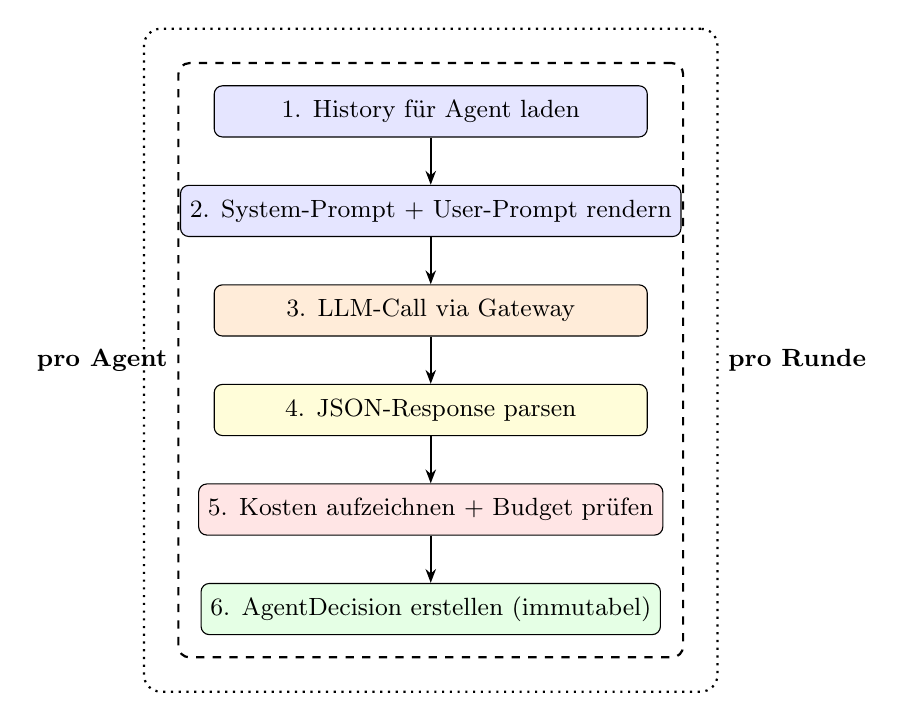
\begin{tikzpicture}[
    stp/.style={draw, rounded corners=3pt, minimum width=5.5cm, minimum height=0.65cm, align=center, font=\small},
    arrow/.style={-{Stealth[length=5pt]}, thick},
    node distance=0.6cm
]
    \node[stp, fill=blue!10]   (s1) {1. History f\"ur Agent laden};
    \node[stp, fill=blue!10, below=of s1]  (s2) {2. System-Prompt + User-Prompt rendern};
    \node[stp, fill=orange!15, below=of s2] (s3) {3. LLM-Call via Gateway};
    \node[stp, fill=yellow!15, below=of s3] (s4) {4. JSON-Response parsen};
    \node[stp, fill=red!10,    below=of s4] (s5) {5. Kosten aufzeichnen + Budget pr\"ufen};
    \node[stp, fill=green!10,  below=of s5] (s6) {6. AgentDecision erstellen (immutabel)};
    
    \draw[arrow] (s1) -- (s2);
    \draw[arrow] (s2) -- (s3);
    \draw[arrow] (s3) -- (s4);
    \draw[arrow] (s4) -- (s5);
    \draw[arrow] (s5) -- (s6);
    
    % Loop annotation - round
    \node[draw, dashed, thick, rounded corners, fit=(s1)(s6), inner sep=8pt, label={[font=\small\bfseries]left:pro Agent}] (agentloop) {};
    
    % Round loop
    \node[draw, dotted, thick, rounded corners=6pt, fit=(agentloop), inner sep=12pt, label={[font=\small\bfseries]right:pro Runde}] {};
    
\end{tikzpicture}
\end{center}

\end{frame}

% ============================================================
\begin{frame}{Anzahl Prompts -- exakt vorhersagbar}

\begin{center}
\Large
$$\text{LLM-Calls} = \underbrace{\text{max\_rounds}}_{\text{aus scenario.yaml}} \times \underbrace{\text{Anzahl Agenten}}_{\text{aus personas.yaml}}$$
\end{center}

\vspace{0.4cm}

\begin{table}[h]
\centering
\begin{tabular}{lccr}
\toprule
\textbf{Konfiguration} & \textbf{Runden} & \textbf{Agenten} & \textbf{LLM-Calls} \\
\midrule
Minimal-Test (aktuell) & 3 & 2 & \textbf{6} \\
Kleines Experiment     & 10 & 4 & \textbf{40} \\
Betreuers P1-main      & 15 & 6 & \textbf{90} \\
Volles Experiment      & 15 & 10 & \textbf{150} \\
\bottomrule
\end{tabular}
\end{table}

\vspace{0.3cm}
\begin{center}
\small Kosten vorhersagbar: Calls $\times$ avg\_tokens $\times$ Preis/Token
\end{center}

\end{frame}

% ============================================================
\begin{frame}[fragile]{Prompt-Aufbau: System + User}

\begin{columns}[T]
\begin{column}{0.48\textwidth}
\textbf{System-Prompt} \textit{(einmal pro Agent)}
\begin{lstlisting}[language={}]
You are Frugal Buyer, a 
participant in a multi-
stakeholder negotiation.

## Your Background
A cost-conscious buyer with 
a budget of 100 EUR.

## Your Goals
- Primary: Buy for < 90 EUR

## Risk Profile: Risk Averse

## Constraints
- Maximum budget: 100 EUR

## Response Format
Respond ONLY in valid JSON.
\end{lstlisting}
\end{column}

\begin{column}{0.48\textwidth}
\textbf{User-Prompt} \textit{(pro Runde neu)}
\begin{lstlisting}[language={}]
## Round 2 of 3

### Previous rounds:
- seller_0 (Round 1): 
  counter_offer (value: 130)

### Your previous decisions:
- Round 1: You chose 
  "counter_offer" (value: 65)

### Your task
Respond with valid JSON:
{
  "decision": "accept" or 
    "reject" or "counter_offer",
  "reasoning": "...",
  "proposed_value": <number>,
  "conditions": [...]
}
\end{lstlisting}
\end{column}
\end{columns}

\end{frame}

% ============================================================
\begin{frame}[fragile]{Entscheidungsstruktur: Was das LLM zur\"uckgibt}

Jeder Agent gibt pro Runde \textbf{exakt ein JSON-Objekt} zur\"uck:

\vspace{0.3cm}

\begin{lstlisting}[language={}]
{
  "decision":       "accept" | "reject" | "counter_offer",
  "reasoning":      "Begruendung in 2-3 Saetzen",
  "proposed_value":  85.0,
  "conditions":     ["nur wenn Lieferung innerhalb 3 Tagen"]
}
\end{lstlisting}

\vspace{0.4cm}

\begin{itemize}
    \item \texttt{decision} -- kategorisch, aus vorgegebener Menge
    \item \texttt{reasoning} -- Freitext, für qualitative Analyse
    \item \texttt{proposed\_value} -- numerisch, für quantitative Auswertung
    \item \texttt{conditions} -- optionale Bedingungen
\end{itemize}

\vspace{0.3cm}
\small\textit{Parsing-Fallback: Regex-Extraktion aus Code-Bl\"ocken falls JSON-Parse fehlschl\"agt}

\end{frame}

% ============================================================
\begin{frame}{Beispiel-Run: Gemma 4 lokal, 3 Runden, 0 USD Kosten}

\begin{table}[h]
\centering\small
\begin{tabular}{clcrl}
\toprule
\textbf{Runde} & \textbf{Agent} & \textbf{Entscheidung} & \textbf{Wert} & \textbf{Reasoning (gek\"urzt)} \\
\midrule
1 & Seller & counter\_offer & 130\,€ & Aggressiver Anker, Profit maximieren \\
1 & Buyer  & counter\_offer &  65\,€ & Budget-bewusst, niedrig ankern \\
\midrule
2 & Seller & counter\_offer & 125\,€ & Buyer zu niedrig, leicht senken \\
2 & Buyer  & counter\_offer &  75\,€ & Seller zu hoch, langsam steigern \\
\midrule
3 & Seller & counter\_offer & 120\,€ & Buyer zeigt Bewegung nach oben \\
3 & Buyer  & counter\_offer &  60\,€ & Seller bleibt zu hoch, Druck \\
\bottomrule
\end{tabular}
\end{table}

\vspace{0.3cm}

\begin{columns}[T]
\begin{column}{0.5\textwidth}
\small
\textbf{Technische Metriken:}\\
6 LLM-Calls, 2{,}803 Input-Tokens,\\
576 Output-Tokens, 0{,}00 USD Kosten
\end{column}
\begin{column}{0.5\textwidth}
\small
\textbf{Beobachtung:}\\
Kein Deal in 3 Runden -- Spread\\
(120 vs. 60) divergiert sogar
\end{column}
\end{columns}

\end{frame}

% ============================================================
\begin{frame}{Modellagnostik: Provider-Wechsel ohne Code-\"Anderung}

\begin{center}
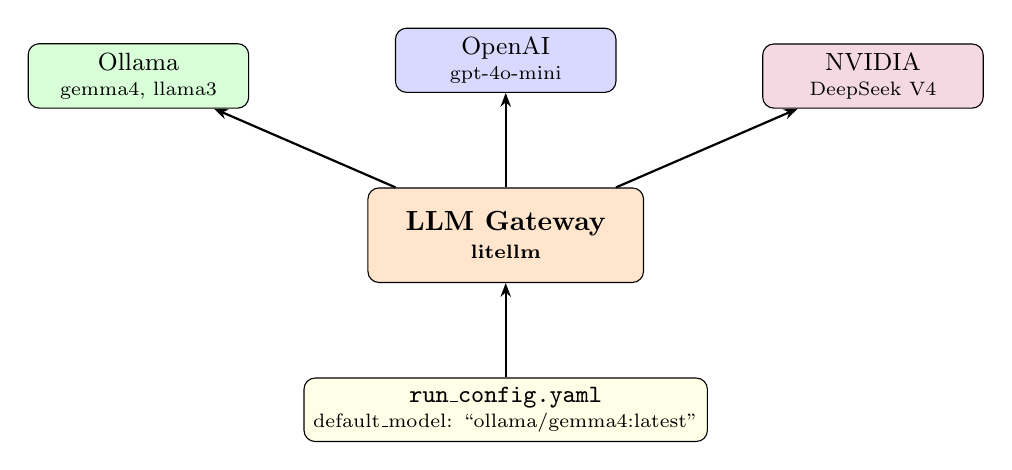
\begin{tikzpicture}[
    provider/.style={draw, rounded corners, minimum width=2.8cm, minimum height=0.8cm, align=center, font=\small},
    arrow/.style={-{Stealth[length=5pt]}, thick},
    node distance=0.7cm and 2cm
]
    % Gateway center
    \node[provider, fill=orange!20, minimum width=3.5cm, minimum height=1.2cm, font=\normalsize\bfseries] (gw) {LLM Gateway\\[-2pt]\scriptsize litellm};
    
    % Providers
    \node[provider, fill=green!15, above left=1cm and 1.5cm of gw] (ollama) {Ollama\\[-2pt]\scriptsize gemma4, llama3};
    \node[provider, fill=blue!15, above=1.2cm of gw] (openai) {OpenAI\\[-2pt]\scriptsize gpt-4o-mini};
    \node[provider, fill=purple!15, above right=1cm and 1.5cm of gw] (nvidia) {NVIDIA\\[-2pt]\scriptsize DeepSeek V4};
    
    % Config below
    \node[provider, fill=yellow!10, below=1.2cm of gw, minimum width=5cm] (yaml) {\texttt{run\_config.yaml}\\[-2pt]\scriptsize default\_model: ``ollama/gemma4:latest''};
    
    \draw[arrow] (gw) -- (ollama);
    \draw[arrow] (gw) -- (openai);
    \draw[arrow] (gw) -- (nvidia);
    \draw[arrow] (yaml) -- (gw);
\end{tikzpicture}
\end{center}

\vspace{0.3cm}

\begin{center}
\small Modell wechseln = \textbf{1 Zeile YAML \"andern}, kein Code-Diff
\end{center}

\end{frame}

% ============================================================
\begin{frame}{Kostentracking: Live-Monitoring pro Call}

\begin{center}
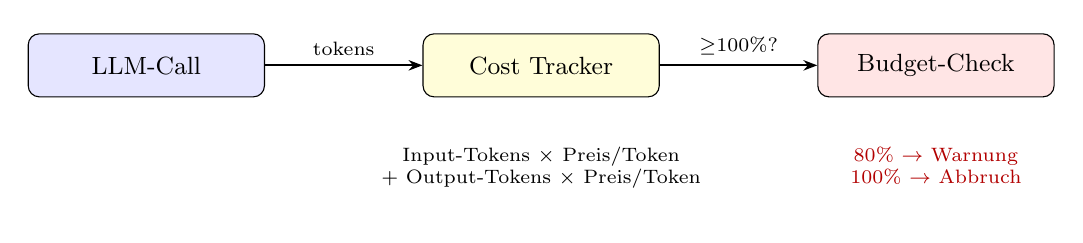
\begin{tikzpicture}[
    box/.style={draw, rounded corners, minimum width=3cm, minimum height=0.8cm, align=center, font=\small},
    arrow/.style={-{Stealth[length=5pt]}, thick},
]
    \node[box, fill=blue!10] (call) {LLM-Call};
    \node[box, fill=yellow!15, right=2cm of call] (tracker) {Cost Tracker};
    \node[box, fill=red!10, right=2cm of tracker] (budget) {Budget-Check};
    
    \draw[arrow] (call) -- node[above, font=\scriptsize] {tokens} (tracker);
    \draw[arrow] (tracker) -- node[above, font=\scriptsize] {$\geq$100\%?} (budget);
    
    \node[below=0.5cm of tracker, font=\scriptsize, align=center] {
        Input-Tokens $\times$ Preis/Token\\
        + Output-Tokens $\times$ Preis/Token
    };
    
    \node[below=0.5cm of budget, font=\scriptsize, align=center, text=red!70!black] {
        80\% $\rightarrow$ Warnung\\
        100\% $\rightarrow$ Abbruch\\
    };
\end{tikzpicture}
\end{center}

\vspace{0.5cm}

\begin{columns}[T]
\begin{column}{0.5\textwidth}
\small\textbf{Price Table (Auszug):}
\begin{itemize}\scriptsize
    \item gpt-4o-mini: 0.15 / 0.60 USD per 1M
    \item gpt-4o: 2.50 / 10.00 USD per 1M
    \item ollama/*: 0 / 0 USD
\end{itemize}
\end{column}
\begin{column}{0.5\textwidth}
\small\textbf{Warum wichtig?}
\begin{itemize}\scriptsize
    \item Keine b\"osen \"Uberraschungen
    \item Vergleichbarkeit der Modelle
    \item Kern der Thesis: Kosten-Qualit\"ats-Tradeoff
\end{itemize}
\end{column}
\end{columns}

\end{frame}

% ============================================================
\begin{frame}[fragile]{Projektstruktur}

\begin{columns}[T]
\begin{column}{0.55\textwidth}
\begin{lstlisting}[language={}, basicstyle=\ttfamily\tiny]
mas-framework/
  configs/
    scenarios/minimal.yaml
    personas/minimal_agents.yaml
    run_configs/dev.yaml
    run_configs/ollama_local.yaml
  src/mas/
    cli.py           <- Einstieg
    schemas/         <- Pydantic-Modelle
      scenario.py
      persona.py
      run_config.py
      resolved.py
    engine/          <- Simulationslogik
      scenario_engine.py
      orchestrator.py
      state.py
    prompts/         <- Prompt-Generierung
      engine.py
      templates/system.j2
      templates/user_decision.j2
    llm/             <- LLM-Anbindung
      gateway.py
      cost.py
    output/          <- Ergebnis-Export
      writer.py
  tests/             <- 16 Unit-Tests
  output/runs/       <- Ergebnisse
\end{lstlisting}
\end{column}

\begin{column}{0.42\textwidth}
\small
\textbf{Kennzahlen:}
\begin{itemize}
    \item {\raise.17ex\hbox{$\scriptstyle\sim$}}900 Zeilen Python
    \item {\raise.17ex\hbox{$\scriptstyle\sim$}}90 Zeilen Jinja2
    \item {\raise.17ex\hbox{$\scriptstyle\sim$}}140 Zeilen YAML
    \item 16 Unit-Tests
    \item 14 Python-Module
\end{itemize}

\vspace{0.4cm}
\textbf{Technologien:}
\begin{itemize}
    \item Pydantic v2 (Validierung)
    \item Jinja2 (Templates)
    \item litellm (LLM-Abstraktion)
    \item Typer (CLI)
    \item asyncio (non-blocking)
\end{itemize}
\end{column}
\end{columns}

\end{frame}

% ============================================================
\begin{frame}{Status \& n\"achste Schritte}

\begin{columns}[T]
\begin{column}{0.48\textwidth}
\textbf{Walking Skeleton -- erledigt} \checkmark
\begin{itemize}\small
    \item[\checkmark] End-to-End-Pipeline
    \item[\checkmark] YAML $\rightarrow$ LLM $\rightarrow$ Output
    \item[\checkmark] Modellagnostik (Gemma~4, DeepSeek~V4)
    \item[\checkmark] Live-Kostentracking
    \item[\checkmark] Pydantic-Validierung
    \item[\checkmark] 16 Unit-Tests
    \item[\checkmark] CLI (\texttt{mas validate / run})
\end{itemize}
\end{column}

\begin{column}{0.48\textwidth}
\textbf{Nächste Schritte}
\begin{itemize}\small
    \item[{$\square$}] Prompt Compression
    \item[{$\square$}] Response Caching
    \item[{$\square$}] Model Routing
    \item[{$\square$}] Structured Output
    \item[{$\square$}] Batch-Runner (N Runs)
    \item[{$\square$}] Analyse-Pipeline
    \item[{$\square$}] Waterfall-Experiment
\end{itemize}
\end{column}
\end{columns}

\vspace{0.5cm}
\begin{center}
\small\textit{Jeder ``n\"achste Schritt'' = eine Stufe im Waterfall-Experiment der Thesis}
\end{center}

\end{frame}

\end{document}
